\chapter{Medida de rendimiento y energía}
\label{chap:medida}
\label{chap:rendimiento}

\section{Qué se está midiendo}

Antes de comparar resultados, mantén fijos el modelo, los datos y la configuración de
ejecución. Anota también el modo de reloj, el modo de mapeo y el número de repeticiones.


\section{Medida de latencia}

La herramienta mide el tiempo empleado por la llamada de ejecución del modelo. La medida
incluye la comunicación entre el host y la tarjeta, la llamada al SDK y la inferencia en
la AKD1000.

La carga de los archivos, el mapeo del modelo y las ejecuciones de calentamiento se realizan
antes de comenzar a medir.

\begin{figure}[H]
  \centering
  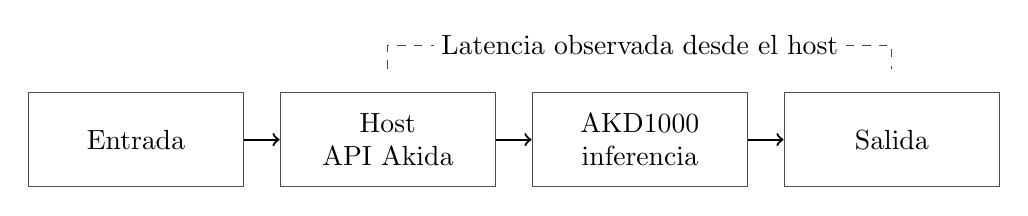
\begin{tikzpicture}[
    stage/.style={draw=black!70,align=center,
                  minimum height=12mm,text width=25mm,fill=white},
    flow/.style={->,thick,draw=black}
  ]
    \node[stage] (input) at (-4.8,0) {Entrada};
    \node[stage] (host) at (-1.6,0) {Host\\API Akida};
    \node[stage] (device) at (1.6,0) {AKD1000\\inferencia};
    \node[stage] (output) at (4.8,0) {Salida};

    \draw[flow] (input) -- (host);
    \draw[flow] (host) -- (device);
    \draw[flow] (device) -- (output);

    \draw[dashed,black!70]
      (-1.6,0.9) -- (-1.6,1.2) -- (4.8,1.2) -- (4.8,0.9);

    \node[fill=white,inner sep=1mm] at (1.6,1.2)
      {Latencia observada desde el host};
  \end{tikzpicture}

  \caption[Frontera de la medida de latencia]
  {Elementos incluidos en la medida de latencia realizada desde el host.}
  \label{fig:measurement-boundary}
\end{figure}

Por tanto, los resultados de este manual se expresan como
\emph{latencia observada desde el host}. No corresponden a un temporizador interno aislado
del AKD1000.

Si se quiere medir el tiempo completo de una aplicación, deben añadirse también las etapas
de adquisición, preprocesado y postprocesado.

\section{Ejecutar un benchmark}

Antes de una campaña completa, ejecuta una prueba corta para comprobar que el
modelo, los datos y la configuración son correctos.

\begin{lstlisting}[language=bash]
akd1000-bringup benchmark \
  --model models/model.fbz \
  --input data/inputs.npy \
  --method forward \
  --clock Performance \
  --map AllNps \
  --warmup 8 \
  --repetitions 1 \
  --output outputs/smoke
\end{lstlisting}

La carpeta de salida contiene:

\begin{itemize}
  \item \code{latencies.csv}, con las medidas individuales;
  \item \code{summary.json}, con la configuración y el resumen del ensayo;
  \item \code{host.json}, con información del sistema utilizado.
\end{itemize}

Comprueba que el número de muestras, las unidades y la configuración son los esperados.
Si la prueba es correcta, repite el benchmark con el número de repeticiones necesario y
guarda los resultados en una carpeta distinta.

Para comparar configuraciones, cambia una sola variable cada vez. Por ejemplo, puedes
mantener fijo el modelo y comparar los modos \code{AllNps}, \code{HwPr} y \code{Minimal},
o mantener fijo el mapeo y cambiar el modo de reloj.

\section{Potencia y energía}

Akida permite habilitar la medida de potencia del dispositivo y consultar las estadísticas
después de una inferencia \cite{brainchip_akida_guide}:

\begin{lstlisting}[language=Python]
device.soc.power_measurement_enabled = True

model.forward(data)

print(model.statistics)
\end{lstlisting}

La potencia proporcionada por esta API corresponde a la medida disponible en el dispositivo.
No representa el consumo completo de la Raspberry Pi, el carrier y la tarjeta.

Con una potencia media y la latencia medida desde el host, puede calcularse
una energía estimada por inferencia como

\begin{equation}
  E_{\mathrm{est}} \,[\mu\mathrm{J}]
  =
  P_{\mathrm{API}} \,[\mathrm{mW}]
  \,
  t_{\mathrm{host}} \,[\mathrm{ms}].
\end{equation}

La relación de unidades es directa:

\[
1\,\mathrm{mW}\cdot 1\,\mathrm{ms}
=
1\,\mu\mathrm{J}.
\]

Esta estimación combina la potencia de la API con la latencia observada desde el host.
Permite comparar ejecuciones con el mismo procedimiento; no mide la energía interna
del chip ni el consumo energético total del sistema.

Para medir el consumo completo sería necesario utilizar instrumentación externa sobre la
alimentación del montaje.

\section{Guardar los resultados}

Para cada ensayo conserva, como mínimo:

\begin{itemize}
  \item el modelo y su versión;
  \item los datos utilizados;
  \item el modo de reloj;
  \item el modo de mapeo;
  \item el número de repeticiones;
  \item los archivos generados por el benchmark.
\end{itemize}

Si se comparan distintas plataformas, como CPU, GPU o FPGA, deben utilizarse la misma tarea,
los mismos datos y una definición equivalente de la medida.
